\section{Build system}
\begin{frame}[t]
	\center{\huge{Construire son système}}
	\begin{figure}
		 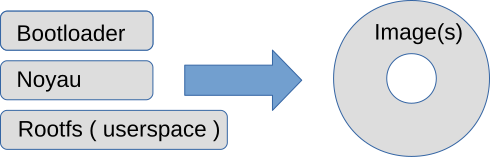
\includegraphics[height=1.5cm]{img/build.png}
	\end{figure}
	\vspace{-1.1cm} % #propreté
	\begin{columns}[t]
	\begin{column}{0.45\textwidth}
	\uncover<2->{\center{Non merci !}}
	\begin{block}<3->{Distribution classique}
		\begin{itemize}
			\item Simple
			\item Pas flexible
			\item Pas optimisé
			\item Architectures classiques
		\end{itemize}
	\end{block}
	\end{column}
	\begin{column}{0.45\textwidth}
	\uncover<4->{\center{Trop facile !}}
	\begin{block}<5->{À la main}
		\begin{itemize}
			\item Flexible
			\item Pas reproductible
			\item Pas maintenable
			\item Pas de dépendances
		\end{itemize}
	\end{block}
	\end{column}
	\end{columns}
\end{frame}
\begin{frame}
	\center{\huge{Build system}}
	\begin{itemize}
		\item<1-> Configure, construit et package les composants
		\item<2-> Gère les dépendances
		\item<3-> Permet la reproductibilité
	\end{itemize}
\begin{block}<4->{Choix critique}
	\begin{itemize}
		\item<5-> Conditionne le développement
		\item<6-> Conditionne l'évolution du projet
		\item<7-> Conditionne les livrables
	\end{itemize}
\end{block}
\end{frame}
% schema
\subsection{Buildroot}
\begin{frame}
	\center{\huge{Buildroot}}
\end{frame}
% buildroot
\subsection{Yocto}
% yocto
\begin{frame}
	\center{\huge{Yocto project}}
	\begin{block}{Principes}
		\begin{itemize}
			\item Groupes de composants réusilisables : Layers
			\item Scripts surchargeables : Recipes
			\item Grosse base de composants
		\end{itemize}
	\end{block}
	\begin{itemize}
		\item Gros projet
		\item Cartes avec variantes
		\item Difficile à prendre en main
	\end{itemize}
\end{frame}
